
\documentclass[11pt,fleqn]{article} 
\usepackage[margin=0.8in, head=0.8in]{geometry} 
\usepackage{amsmath, amssymb, amsthm}
\usepackage{fancyhdr} 
\usepackage{palatino, url, multicol}
\usepackage{graphicx, pgfplots} 
\usepackage[all]{xy}
\usepackage{polynom} 
%\usepackage{pdfsync} %% I don't know why this messes up tabular column widths
\usepackage{enumerate}
\usepackage{framed}
\usepackage{setspace}
\usepackage{array,tikz}

\pgfplotsset{compat=1.6}

\pgfplotsset{soldot/.style={color=black,only marks,mark=*}} \pgfplotsset{holdot/.style={color=black,fill=white,only marks,mark=*}}


\pagestyle{fancy} 
\lfoot{}
\rfoot{\S 2.2}

\begin{document}
\renewcommand{\headrulewidth}{0pt}
\newcommand{\blank}[1]{\rule{#1}{0.75pt}}
\newcommand{\bc}{\begin{center}}
\newcommand{\ec}{\end{center}}
\renewcommand{\d}{\displaystyle}

\vspace*{-0.7in}

%%%%%%%%%intro page
\begin{center}
  \large
  \sc{Section 2.3: Volumes of Revolution using Cylindrical Shells}\\
\end{center}

\begin{enumerate}
\item In the space below, write the formulas for the Disk Method and the Washer Method with accompanying formulas. Assume we are integrating with respect to $x.$\\
\vfill

\item Sketch the region $R$ bounded by $y=\frac{1}{1+x^2}$, $y=0$, $x=0$, and $x=2.$ (The graph of $y=\frac{1}{1+x^2}$ is sketched for you below.) We want to determine the volume of the solid obtained by rotating $R$ about the $y$-axis. \\

\begin{center}
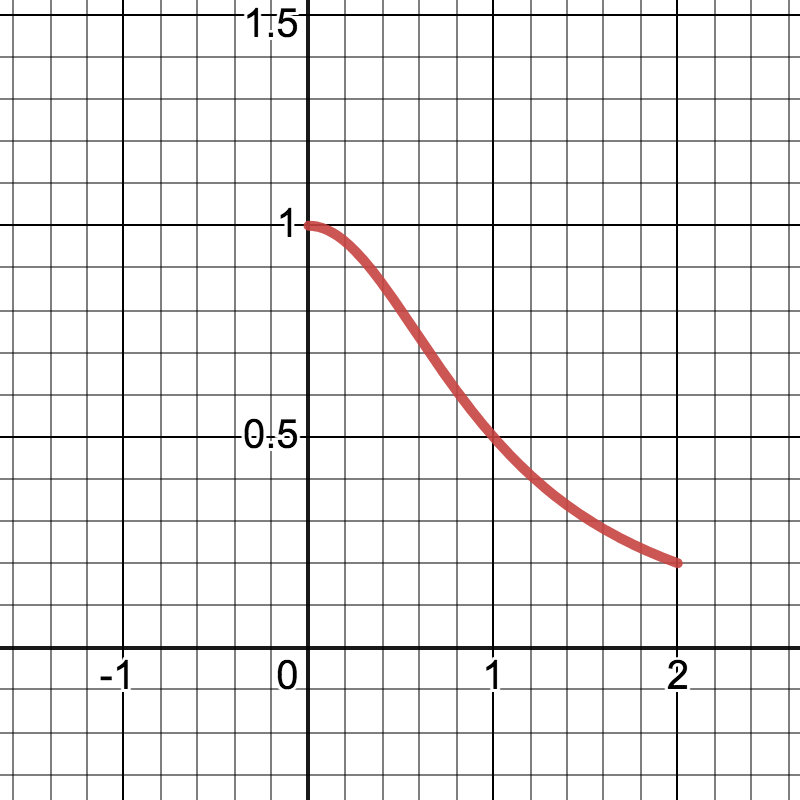
\includegraphics[scale=0.2]{pic-2-3-a.png} 
\end{center}

\begin{enumerate}
\item If we wanted to use the Disk Method, how would we slice the region $R$? Explain why this choice would be inconvenient?

\vspace{.6in}

\item Slice the region $R$ vertically and sketch the shape that slice would make on the figure above. Describe the shape in words.\\

\vspace{.6in}

\item In the space below, we will set up and evaluate the integral for the volume of this solid.

\vfill

\end{enumerate}
\newpage
\item Determine the formula for the volume of a cylindrical shell.
\vspace{1in}
\item Use the formula for the volume of a cylindrical shell, to deduce the Method of Cylindrical Shells formula. Draw an accompanying picture.
\vfill
\item Sketch the region bounded above by $y=e^{x^2}$, below by $y=1-x,$ and on the right by $x=1.$ Use the Method of Cylindrical Shells to find the volume of the solid obtained by rotating $R$ about the $y$-axis. (Note $y=e^{x^2}$ is already graphed for you below.)

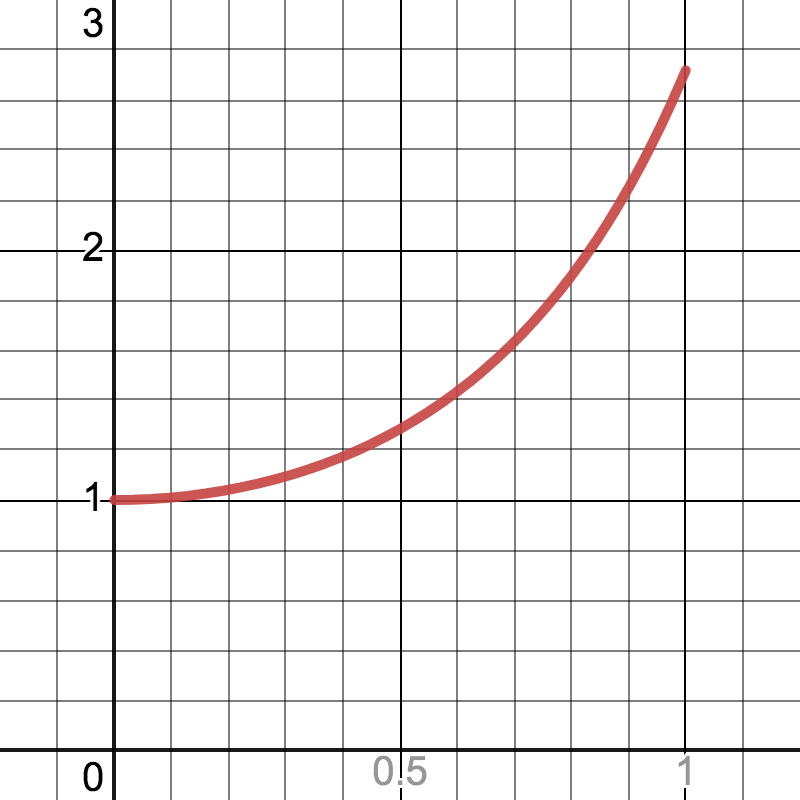
\includegraphics[scale=0.2]{pic-2-3-b.png} 
\vfill
\item Repeat the problem 5, but slice the region horizontally and use disks/washers. 
\vspace{1in}

\end{enumerate}
\end{document}

